\fancychapter{State of the art}
%TODO write that the state of the art is divided in basic concepts and actual state of the art
\section{Basic Concepts} 
\label{sec:basic_concepts}

In this Section we will start by generally describing what Clustering is and how it works then we will outline how Self-Organizing maps ~\cite{Kohonen1990} function, which is the Document Clustering algorithm used on this project.

\subsection{Document}
\label{sub:clustering}
Document clustering is an optimal division of documents into categories without prior knowledge of the data that is being organized, based only on the similarity between them. Due to the fact that no prior knowledge of the data has to be known Document Clustering is labeled as Unsupervised Machine Learning.

Yuan-Chao Liu et Al ~\cite{Liu2012b} asserted that Document Clustering can be used in a variety of Computer Science fields, such as:
\begin{itemize}
  \item Natural Language Preprocessing.
  \item Automatic Summarization.
  \item User preference mining.
  \item Improving text classification results.
\end{itemize}

There are two main types of Document Clustering, Hard Clustering and Soft Clustering. In Hard Clustering one document can only belong to one cluster, while in Soft Clustering one document can belong to multiple clusters. 

In regard to document categorization ~\citet{Springorum1998} performed clustering with SOMs ~\citep{Kohonen1990} while identifying polysemous German Propositions. They used regular SOMs to create multiple clusters and used Centroid-Based or Preposition-based softening to create Soft Clusters from the Hard Clusters.

The clustering process usually works as described in ~\ref{fig:1_Text_Clustering_Main_Framwork}
\begin{figure}
  \begin{center}
    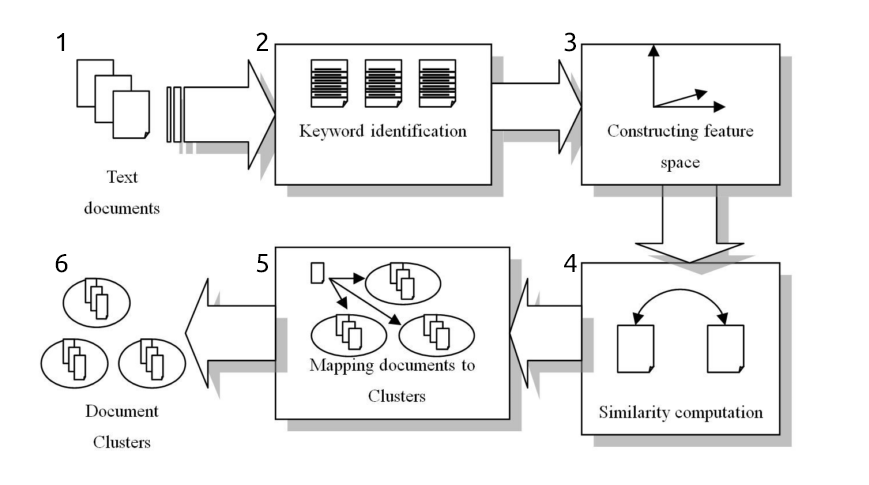
\includegraphics[width=12cm]{images/1_Text_Clustering_Main_Framwork.png}
  \end{center}
  \caption{ Text Clustering Main Framework from ~\citet{Dozono2012} }
  \label{fig:1_Text_Clustering_Main_Framwork}
\end{figure}
In the first, step a data set must be provided in order to cluster the documents. 
The second step is where non relevant words are removed from the documents. ~\citet{Kang2003} proves that improves clustering. Another way to extract keywords is to differentiate text features by analyzing the document corpora. For example if the dataset is composed from HTML or XML documents it is possible to identify more relevant features due to the characteristics of the markup.
The fourth step is characterized by converting the keywords of each document into vectors, the most common model used for this task is VSM (Vector Space Model). In VSM, each vector dimension means one detected keyword and each document is represented by the vector of keywords in the feature space. This process an is described in Figure ~\ref{fig:2_svm}.

\begin{figure}
  \begin{center}
    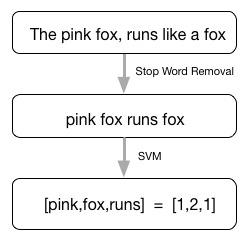
\includegraphics[width=5cm]{images/2_svm.jpg}
  \end{center}
  \caption{ Stop word removal and transformation to Vector Space Model }
  \label{fig:2_svm}
\end{figure}


There many clustering algorithms. K-means works by randomly selecting k documents as the cluster centroids, then assigning each document to the nearest centroid, and finally recalculate the the centroid with new added documents. 

\subsection{The Self-Organizing Map} 
\label{sub:the_self_organizing_map}

The Self-organinzing map, or SOM, is a kind of recurrent artificial neural network that has the desired property of topology preservation which mimics the way the cortex of highly developed animals brains work.

As \citet{Bacao2005} describes, the basic idea behind SOM is to map the data patterns into an n-dimensional grid of neurons or units. That grid is also know as the output space, as opposed to the initial space also called input space, where the input patterns are. Both spaces can be seen in Figure~\ref{fig:5_neighbours_converge}.

SOMs work similar to the way that is thought that the human brain works, by having a set of neurons that through learning experience specialize in the identification of certain types of patterns. These neurons are responsible for categorizing the input patterns for which they are responsible. Nearby neurons will be organized by similarity which will cause that similar patterns will activate similar areas of the SOM.
With a topology preserving mapping, SOM organizes the information spatially where similar concepts are mapped to adjacent areas. The topology is preserved in a sense that, as far as possible, neighborhoods are preserved through the mapping process.
Neurons are displayed in an N dimensional grid, generally rectangular, but other structures are possible, such as hexagonal or octagonal.  The grid of neurons, also called output space, can be divided in neighborhoods, where neurons responsible for the same kind of input reside.
In SOM, neurons will have the same amount of coefficients as the input patterns and can be represented as vectors through the VSM model described earlier in Section ~\ref{sub:clustering}.

Before describing the algorithm it is important to define two key aspects of the SOM, the learning rate and quantization error. The learning rate is a function that will be decreased in order to converge to zero, it will be applied to winning neurons and their neighbors in order for them to move toward the corresponding input pattern. Quantization Error is the distance between a given input pattern and the associated winning neuron, it describes how well neurons represent the input pattern. The radius of the neighborhood around the winner neuron is particularly relevant to the topology of the SOM, deeply affecting the unfolding of the output space as stated by \citep{Bacao2005}.
\par
The learning phase is characterized by the training algorithm, which works the following way:
\begin{itemize}
  \item Neurons can be initialized randomly or it is possible to select a specific initialization.
  \item Given an input pattern, calculate the distance between the input pattern and every neuron on the network.
  \item The winning neuron will be the closest neuron to the input pattern.
  \item The neuron will move towards the data pattern at a given learning rate, in order to improve his representation as can be seen in Figure~\ref{fig:4_wining_neuron_converge}.
  \item Neighbor neurons will also improve their representation in order to keep the network progressively organized as can be seen in Figure~\ref{fig:5_neighbours_converge}.
\end{itemize}

\begin{figure}
  \begin{center}
    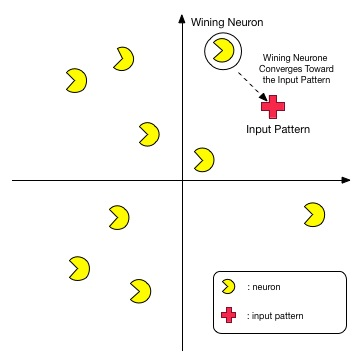
\includegraphics[width=5cm]{images/4_wining_neuron_converge.jpg}
  \end{center}
  \caption{ Winning neuron converging at learning rate }
  \label{fig:4_wining_neuron_converge}
\end{figure}

\begin{figure}
  \begin{center}
    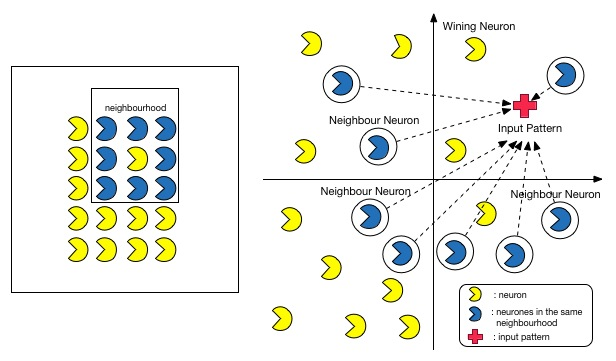
\includegraphics[width=12cm]{images/5_neighbours_converge.jpg}
  \end{center}
  \caption{ On the left the output space neighbor, on the right the neighbors of the winning neuron converging }
  \label{fig:5_neighbours_converge}
\end{figure}

After the algorithm converges, the prediction phase starts. On the prediction phase new input patterns can be quickly assigned to the SOM, without need to apply the learning rate to the winning neuron and his neighbors. Thus it very easy and fast to classify new data now.

In order to visually interpret the result of the SOM U-matrices may be used as stated by ~\citep{Bacao2005}. The U-matrix is a representation of the SOM in which distances, in the input space between neurons is represented using a gray scale.

The advantages of using SOM is data noise immunity, easy to visualize the data, and parallel processing.

\section{Related Work}
\label{sec:related_work}

This Section provides insight of work done in multiple research areas that are related to the project. In subsection ~\ref{sub:self_organizing_maps} will be described multiple work done using Self-Organizing maps. Subsection ~\ref{sub:topic_detection_on_twitter} is dedicated to work done on topic detection on the social network Twitter \footnote{http://www.twitter.com}

\subsection{Self-Organizing Maps} 
\label{sub:self_organizing_maps}
Self-Organizing maps are used in a wide are of applications, from authentication systems ~\cite{Dozono2012} through network intrusion detection ~\cite{intrusion_som} and speech recognition and analysis ~\cite{phonetic_typewiter}.

\subsubsection{The Geo-Som Approach} 
\label{ssub:types_of_soms}
The Geo-SOM ~\citet{Bacao2005} applies the first column of geography “Everything is related to everything else, but near things are more related than distant things." to the SOM algorithm, where the winning neuron is chosen by in a radius k defined by the geo-coordinates of the data. In this way the Geo-som forces units that are close in the input space to be close in the output space. The representation of the Geo-som can be seen in Figure ~\ref{fig:geo_som}.

\begin{figure}[tb]
  \begin{center}
    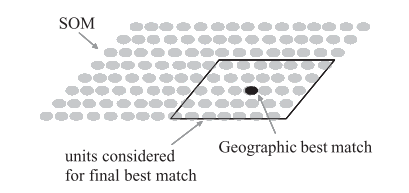
\includegraphics[]{images/6_geo-som.png}
  \end{center}
  \caption{Geo-SOM structure, from ~\citet{Bacao2005}}
  \label{fig:geo_som}
\end{figure}

\subsubsection{Detecting Hidden Patterns on Twitter Usage} 
\label{ssub:detecting_hidden_patterns_on_twitter_usage}
Cheon and Lee ~\citep{Cheong2010} analyzed hidden patterns created buy the natural usage of twitter by its users. In its study they started by collecting data from the twitter API of different kinds of topics like "2009 Iran Election" and "iPhone 3.0 OS launch". They made multi level signal extraction not only from information directly present on the tweet, but also by cross referencing with other social website and with the twitter user profile information. The signals retrieved from the social network can be seen in Table ~\ref{tab:twitter_signals}.

\begin{table}[H]
  \caption{Twitter Signals}
  \label{tab:twitter_signals}
  \begin{center}
    \begin{tabular}{|l|l|l|}
    \hline

    \hline
    \textbf{Twitt Corpus} & \textbf{Twitter Profile} & \textbf{External Sources} \\
    \hline
       Tweet Size & Gender & Other Social Network Accounts\\
    \hline
       Replies & Number of customizations & Type of website\\
    \hline
       Re-tweets & Friends to followers ratio & \\
    \hline
       Hashtags & frequency of posts & \\
    \hline
      \specialcell{Presence of URIs and \\ Type of linked content}
        & Account Age
        & \\
    \hline
       Type of Device & Country & \\
    \hline
       Tweet Location &  & \\
    \hline
    \end{tabular}
  \end{center}
\end{table}

By applying a SOM, they could find 4 demographical clusters during the Iran 2009 Election. The first columnster was characterized by young web-based Iranians, with twitter accounts not older than 3 months with a high frequency of replies. The second cluster was mainly compound of web users from Iran accounts older that 3 months. The third cluster had Iranian users with mobile clients with large texts clearly trying to raise awareness. The fourth and final cluster represented the users around the world trying to raise awareness about the issue by sharing tweets with URIs.
Looking at their analysis about the topic "2009 Iranian Election" it is clear to see that it was possible to describe the type of users represented in the social network and the way they interact with it.

On the iPhone 3.0 OS launch it was possible to find three main clusters. The first columnster was characterized by male users, accounts older than 90 days, coming from countries where the iPhone is marketed, with high adoption of social media clearly representing the target market of the iPhone or its customers. The second cluster had new accounts with higher rate of followers to followees, high frequency of posts per day, presence of URI linking to technology blogs or websites, no country or gender specified meaning that this cluster was clearly composed by news aggregators and technological news websites. Inside the second cluster there was a sub-cluster of Japanese users which represents the high rate of iPhone adoption in Japan. Finally the third cluster was clearly spammer accounts that where eventually deleted after a couple of months, characterized by popular social connections, posting more than 50 tweets a day with external URIs and the accounts where not older than a day or so.

In conclusion it was possible to detect Twitter usage patterns and specifically detect spammers before they where banned from the social network. 

\subsection{Topic Detection and Clustering} 
\label{sub:topic_detection_on_twitter}
There have been many topic detection techniques. Many of them rely on the TF IDF~\cite{Baeza-Yates:1999:MIR:553876} (term frequency – inverse document frequency) which is not particularly adequate for topic detection on Twitter due to the fact that tweets are very small, composed by typos or slang words and might be written in multiple languages, sometimes at the same time. In this subsection we will take a look at multiple methods of topic detection in general and specifically on the Twitter social network.

\subsubsection{Topic and Trending Detection} 
\label{ssub:real_time_topic_and_trending_detection}
Due to the rapid adaptation of people to always be on-line, through the usage of cellphones on the move, desktops at work and even theTV at home, the increase of user generated content has increased tremendously in latest years. In 2006 35\% of on-line adults and 57\% of teenagers created content on the Internet \footnote{ Data source: http://www.pewinternet.org/Presentations/2006/UserGenerated-Content.aspx}, which in "Internet Years" was ages ago.
With amount of content increasing, new real-time and scalable algorithms are needed in order to make sense of all this data.
~\citet{Cataldi2010} propose a new technique for emerging topic detection that permits real-time retrieval of the most emergent topics expressed by a community on Twitter. Their work applies the PageRank ~\cite{Pagerank1998} algorithm to the users follower/followee relationship in order to find the most influential user on the network, and then calculates the most trending topics by relating, social influence, word co-occurrence and time frame. In the end, an interface was created where it would be possible to navigate hot topics in a given time frame. Topic labeling was not automatic and was implicit by the time frame of an event, if two highly social events would occur in the same time frame with word relations the results could be interpreted as the same, for example if a political candidate would win the elections at the same of an important sports club would win a specific cup, the word \emph{win} could be trending at the same time for two different topics and due to high temporal dependency they could be interpreted as the same topic.
~\citet{Weng2010} also used the PageRank algorithm in order to find the most influential twitter users on a certain topic, but uses a different approach where they represent each twitter user as a bag of words comprising of all the tweets that they have posted. Afterwards it uses Latent Dirichlet Allocation ~\cite{Blei2003} in order to find the topics each user is interested in. In the end it was possible to prove that follower/followee relation on twitter was not just casual, but that people actually follow other people in which they have some resemblance or common interest. This concept is called homophily and will be further explored by this project.

\subsection{Data Mining in Twitter } 
\label{sub:data_mining_in_twitter_}
In this subsection, we will focus on work done on the Twitter social network in order to leverage insights on how the public data available from the website can correlated within itself and with outside sources. 

\subsubsection{Enhancing the Tweet} 
\label{ssub:the_tweet}
Tweet retrieval and analysis is a double edged problem. On one side the tweet is really small which makes it almost impossible to retrieve any actual sense from it. On the other hand the amount of tweets generated per day is around 140 million \footnote{https://blog.twitter.com/2011/numbers} wich means that it is very hard to a deep analyses of the semantics and content of individual tweets, and that, only the more appropriate signals should be evaluated.
~\citet{Tao2012} evaluated how the multiple signals that could be retrieved directly or indirectly from the tweet corpus could mean that a tweet is relevant for a determined topic. In his work, Tao presents premises that seem intuitively true and proves they actually are relevant through a comparison of multiple precision and recall values. Its results on feature comparison where summarized in Table ~\ref{tab:tao_table}, the first column consists of all the made hypothesis categorized by type, and the second column tells if the data used actually influenced in precision and recall results. Tau also compared result of topic characteristics, concluding that distinction between local and global events as well as temporal persistence proved to not be relevant on relevance prediction.

\begin{table}[tb]
  \caption{~\citet{Tao2012} resumed results}
  \label{tab:tao_table}
  \begin{tabularx}{\textwidth}{|X|l|}
  \hline
  \textbf{Hypotheses} & \textbf{Influence of Features} \\
  \hline
  \hline

  {\bf Syntatical} &  \\
  \hline
  Tweets that contain hashtags are more likely to be relevant than tweets that don't & Not Important \\
  \hline
  Tweets that contain an URI are more relevant that tweets that don't  &Important \\
  \hline
  Tweets that are replies to other tweets are less relevant & Important \\
  \hline
  The longer the tweet is the more relevant it is & Not Important\\
  \hline
  \hline

  {\bf Semantic}  &  \\
  \hline
  
  The more the number of entities the more relevant a tweet is  & Important \\
  \hline
  Different types of entities are of can have different amount of interest to a give topic  & Important \\
  \hline
  The greater the diversity of concepts mentions in a tweet the more likely for it to be relevant & Important \\
  \hline
  The relevance of a tweet is determined buy its polarity & Important \\
  \hline
  \hline

  {\bf Contextual} &  \\
  \hline
  The lower the temporal distance between a query and the creation of a tweet the more relevant the tweet is  & Not Important \\
  \hline
  The more the number of tweets created by a user the more relevant one of his tweets will be & Not Important \\
  \hline
  \end{tabularx}
\end{table}

~\citet{McCreadie2013} also approached the issue of having very little content on tweets in order to categorize a tweet, and tried to solve it by applying the content of linked URIs into the tweet body in order to improve precision and recall. The best fitting approach was using Field-Based weighting where for each tweet a new document is created which contains two fields; the terms in the tweet and the terms in the linked document. 
Afterwards a learning to rank algorithm called PL2F is used against the dataset from Microblog2011 in order to find the best weighting that should be applied to the tweet corpus and the URI referenced page. 
With this trained model they where able to improve precision in an order of 0.9. 

\subsubsection{Rapidly Changing Trends} 
\label{ssub:real_time_}
Due to the real time nature of Twitter, using typical retrieval model that relies on term frequency models like BM25 or language modeling cannot be applied, as stated by ~\citet{Lin2012}. The study of topic perdurance on the social network proved that it is presented in bursts of queries and mentions of a topic. The typical usage of twitter for search is not the same of Google. When user are searching in twitter they want to find out what is happening right know meaning that classification techniques based on past events cannot respond this kind problem. As stated by ~\citet{Lin2012} this problem has not yet been solved at Twitter (or anywhere else at the time of writing this report), and issues a new kind of data analysis approach that was not taken into consideration in the past. 
This effect of rapidly changing topics and queries based on real time events was named "Churn", and can be clearly seen in Figure ~\ref{fig:churn}.

  \begin{figure}[tb]
    \begin{center}
    \noindent\makebox[\textwidth]{
      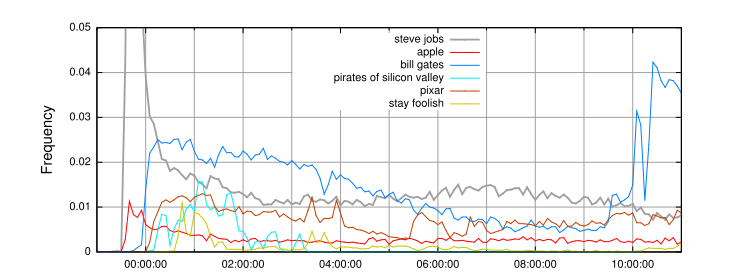
\includegraphics[width=13cm]{images/7_churn.png}
    }
    \end{center}
    \caption{The Churn effect: Frequencies of queries related to Steve Jobs death over a 12 hour period in 5-minute intervals, normalized to the total number of queries in the interval. At its peak, the query “steve jobs” reaches 0.15 (15\% of the query stream); Graph taken from ~\cite{Lin2012}}
    \label{fig:churn}
  \end{figure}


\section{Summary}
%TODO Sumarize the state of the art
Ending section summarizing the chapter is typically a good idea.

Ensure that the next chapter starts in a odd page
\cleardoublepage 
